%GiG
\documentclass{beamer} 
\usetheme{Copenhagen}
\setbeamertemplate{navigation symbols}{}
\setbeamertemplate{headline}{}
\DeclareMathOperator*{\argmax}{arg\,max}

\usepackage{hyperref}


\definecolor{azure}{rgb}{0.0, 0.5, 1.0}
%\newcommand{\tblue}[1]{\textcolor{blue}{#1}}
\newcommand{\tblue}[1]{{\Large {\textcolor{azure}{#1}}}}
\newcommand{\thblue}[1]{{\Huge {\textcolor{azure}{#1}}}}
\newcommand{\hred}[1]{{\textcolor{red}{#1}}}
\newcommand{\furl}[1]{{\footnote{\url{#1}}}}

\newcommand{\mypause}{\pause}
%\newcommand{\mypause}{}

\title[Saravanan Thirumuruganathan] 
{Lecture 4: Data Collection and Munging}

\author[CSE 5334] 
{Instructor: Saravanan Thirumuruganathan}

\date[] 

\begin{document}


\begin{frame}
  \titlepage
\end{frame}

%\begin{frame}{Outline}
%  \tableofcontents
%  % You might wish to add the option [pausesections]
%\end{frame}

\section{Outline}

\begin{frame}
\frametitle {Outline}
\begin{enumerate}
\item Data Collection and Scraping
\item Web Scraping basics
\end{enumerate}
\end{frame}


\begin{frame}{In-Class Quizzes}
\begin{itemize}
\item {\Large {\bf URL:}} {\LARGE \bf \url{http://m.socrative.com/}} 
\item {\Large {\bf Room Name:} {\LARGE \bf 4f2bb99e}}
\end{itemize}
\end{frame}


\section{Data Collection}
\begin{frame}{} 
    \begin{center}
        \thblue{Data Collection}
    \end{center}
\end{frame}

\begin{frame}{What you wish data looked like?}
    \begin{center}
        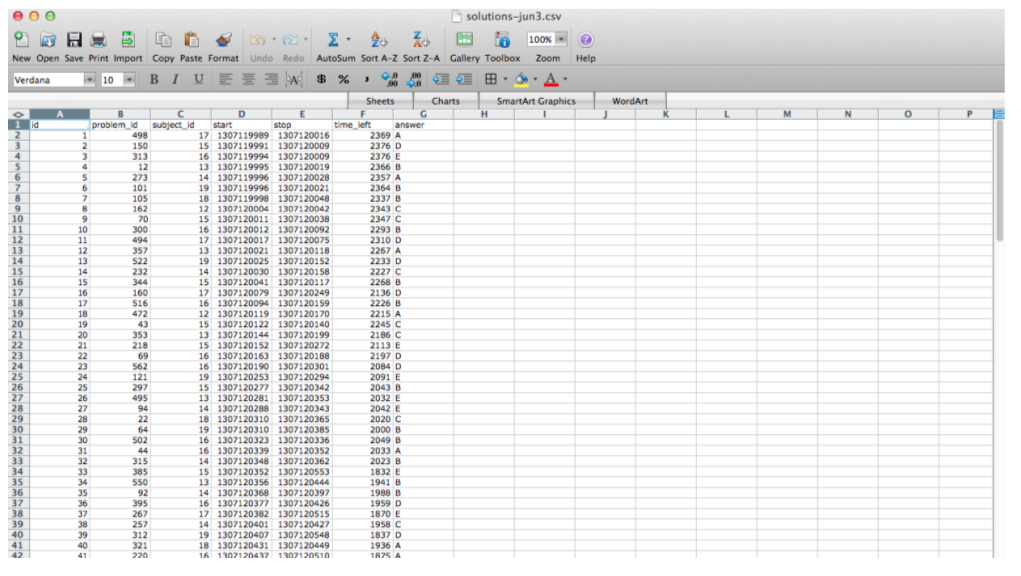
\includegraphics[scale=0.3]{dataIdeal.png}
    \end{center}
\end{frame}
\begin{frame}{What does data really look like?}
    \begin{center}
        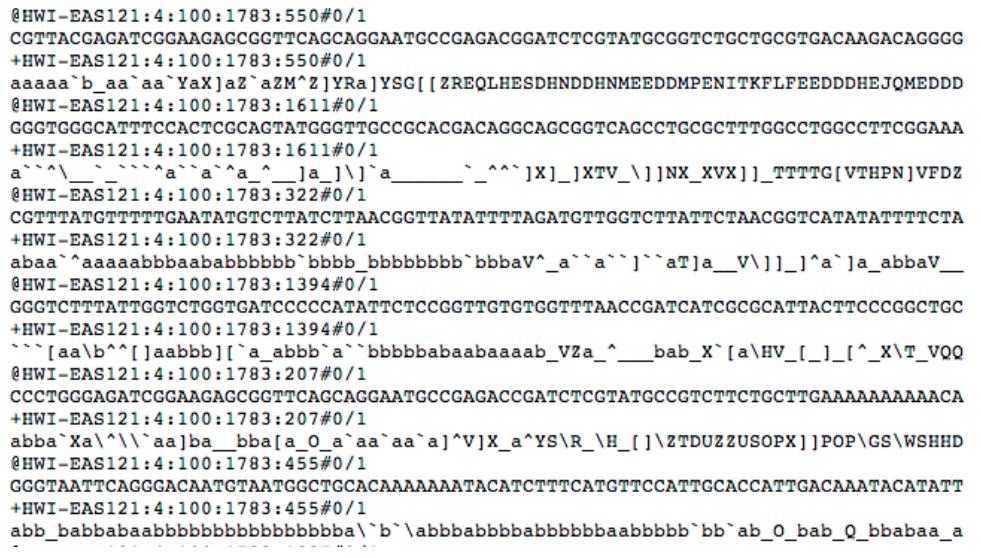
\includegraphics[scale=0.24]{dataActual.png}
    \end{center}
\end{frame}
\begin{frame}{What does data really look like?}
    \begin{center}
        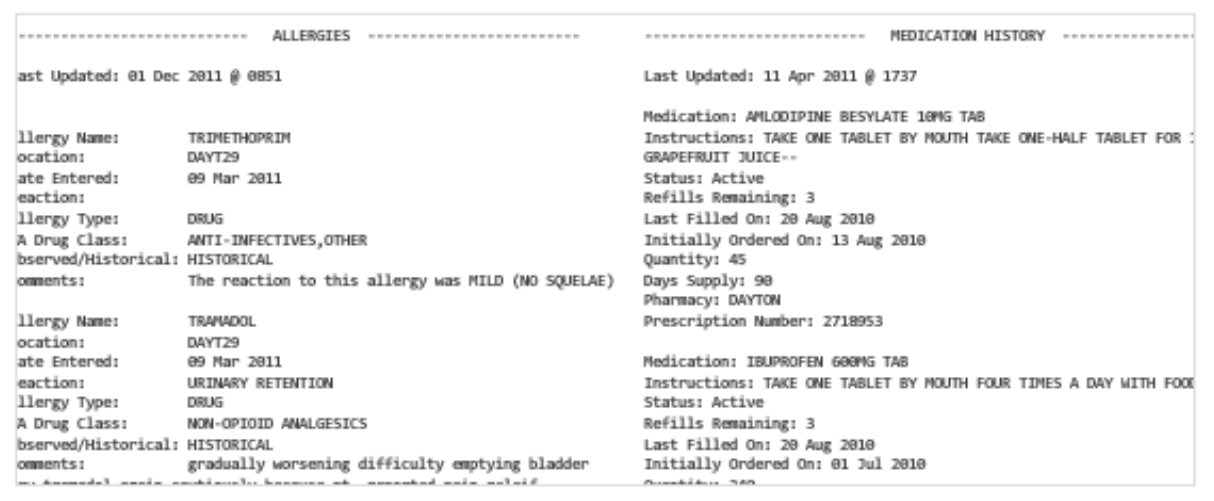
\includegraphics[scale=0.3]{dataActual2.png}
    \end{center}
\end{frame}
\begin{frame}{}
    \begin{center}
        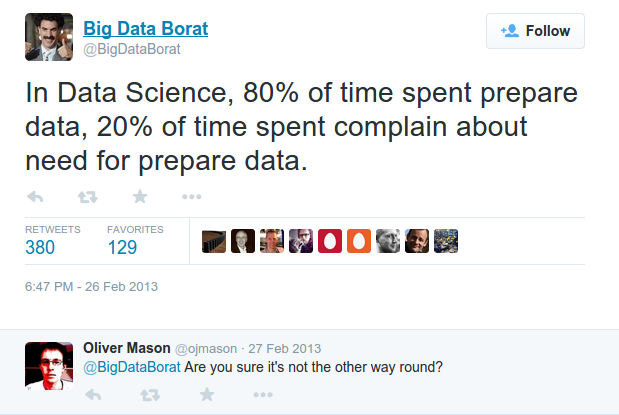
\includegraphics[scale=0.4]{bigDataWork.png}
    \end{center}
\end{frame}
\begin{frame}{What Do Analysts Do?}
    \begin{center}
        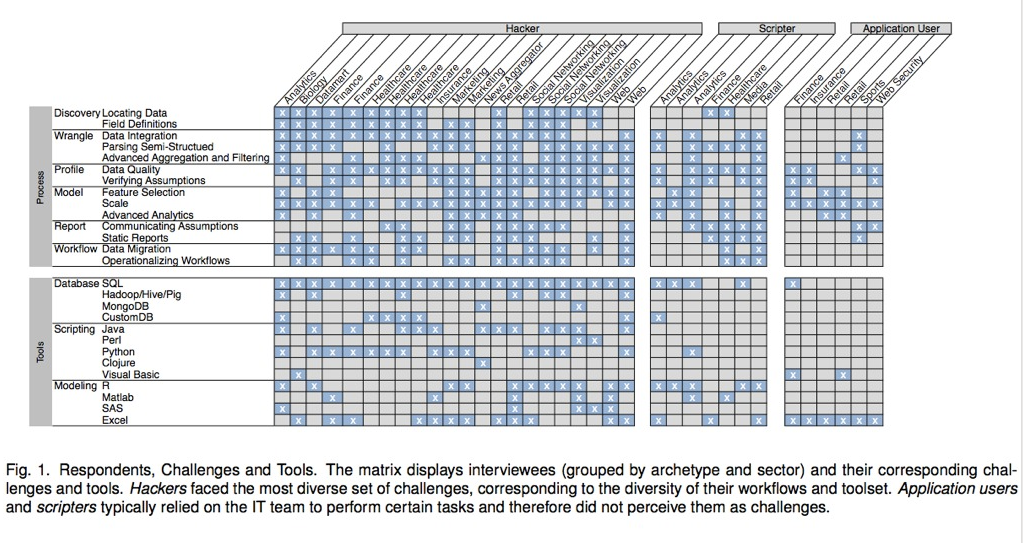
\includegraphics[scale=0.3]{whatDoAnalystsDo.png}
    \end{center}
\end{frame}
\begin{frame}{What Do Analysts Do?}
    \begin{center}
        {\em I spend more than half of my time integrating,
        cleansing and transforming data without doing any
        actual analysis. Most of the time I'm lucky if I get to
        do any analysis. Most of the time once you transform
        the data you just do an average... the insights can be
        scarily obvious. It's fun when you get to do something
        somewhat analytical.}
    \end{center}
\end{frame}


\begin{frame}{Data Collection Ethics}
    \begin{itemize}
        \item OK: Public, non-sensitive, anonymized, fully referenced information (always cite sources)
        \item If in doubt, don't!
        \item Be a good web citizen: 
        \begin{itemize}
            \item Honor robots.txt
            \item Obey rate limits. Do not overload servers
            \item Obey relevant copyright/license restrictions
            \item Know about fair use and its restrictions
        \end{itemize}
    \end{itemize}
\end{frame}

\begin{frame}{Data Collection: 4 Things You Should Have}
    \begin{enumerate}
        \item Raw data
        \item Tidy data set
        \item A code/process book describing each variable and its values in tidy data set
        \item A explicit and exact recipe you used to go from $1$ to $2,3$.
    \end{enumerate}
\end{frame}


\begin{frame}{Tidy Data}
    \begin{enumerate}
        \item Each variable you measure should be in one column
        \item Each different observation of that variable should be in a different row
        \item There should be one table for each ``kind'' of variable
        \item If you have multiple tables, they should include a column in the table that allows them to be linked
    \end{enumerate}
    Other Tips:
    \begin{itemize}
        \item Include a row at top of each file with variable names
        \item Make variable names human readable AgeAtDiagnosis instead of AgeDx
        \item In general, data should be saved in one file per table
    \end{itemize}
\end{frame}

\begin{frame}{Why is the instruction list important?}
    \begin{center}
        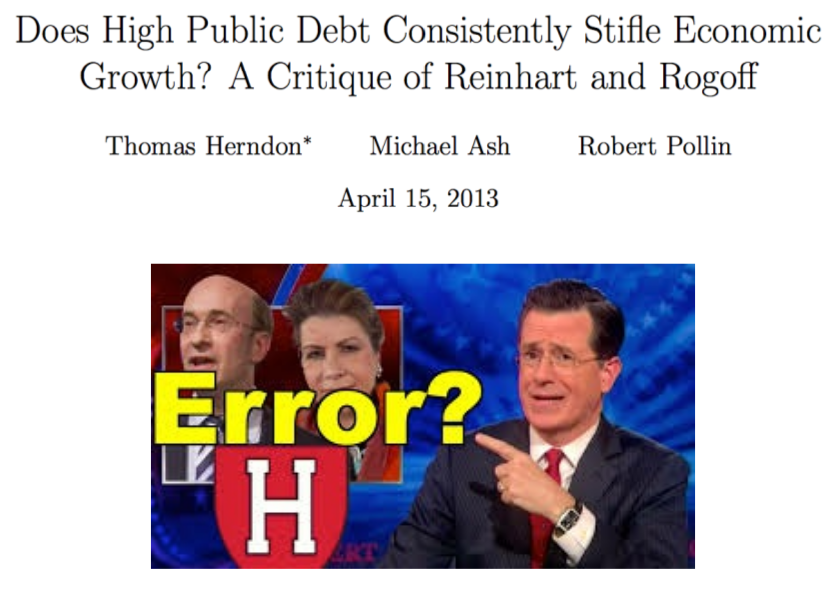
\includegraphics[scale=0.35]{rogoff.png}
    \end{center}
\end{frame}
\begin{frame}{Why is the instruction list important?\furl{http://telegraph.co.uk}}
    \begin{center}
        
\includegraphics[scale=0.35]{piketty-capital-21st-century.jpg}
    \end{center}
\end{frame}

\begin{frame}{Data Access Schemes}
    \begin{itemize}
        \item {\bf Bulk downloads:} Wikipedia, IMDB, Million Song Database, etc. See list of data web sites on the Resources page
        \item {\bf API access:} NY Times, Twitter, Facebook, Foursquare, Google, ...
        \item {\bf Web scraping:} For everything else
    \end{itemize}
\end{frame}


\begin{frame}{Data Formats}
    \begin{itemize}
        \item Delimited Values
        \begin{itemize}
            \item Comma Separated Values (CSV)
            \item Tab Separated Values (TSV)
        \end{itemize}
        \item Markup Languages
        \begin{itemize}
            \item Hypertext Markup Language (HTML / XML)
            \item JavaScript Object Notation (JSON)
            \item Hierarchical Data Format (HDF5)
        \end{itemize}
        \item Ad Hoc Formations
        \begin{itemize}
            \item Graph edge lists, voting records, fixed width files, ...
        \end{itemize}
    \end{itemize}
\end{frame}


\begin{frame}{JSON}
    \begin{itemize}
        \item Light weight text-based interchange format
        \item Language independent 
        \item Based on Javascript
        \item Very easy to use and manipulate
        \item All browsers and major languages have great support
    \end{itemize}
\end{frame}


\begin{frame}{JSON}
    \begin{itemize}
        \item A collection of name/value pairs: \\ \qquad \qquad $\{``a":1, ``b":2,``c":3,``d":4,\}$
        \item An ordered list of values:\\ \qquad \qquad  $[1,2,3,``blah"]$
        \item Or a combination: \\ \qquad \qquad $\{ ``a": [1,2,3,4], ``b": [5,6,7,8], ``c": 4 \}$
    \end{itemize}
\end{frame}


\begin{frame}{XML}
    \begin{center}
        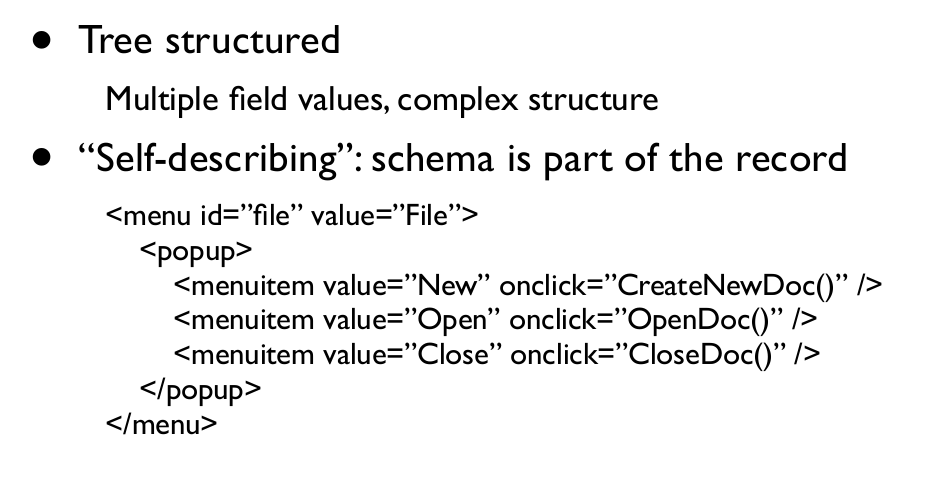
\includegraphics[scale=0.3]{xml.png}
    \end{center}
\end{frame}
\begin{frame}{HTML}
    \begin{center}
        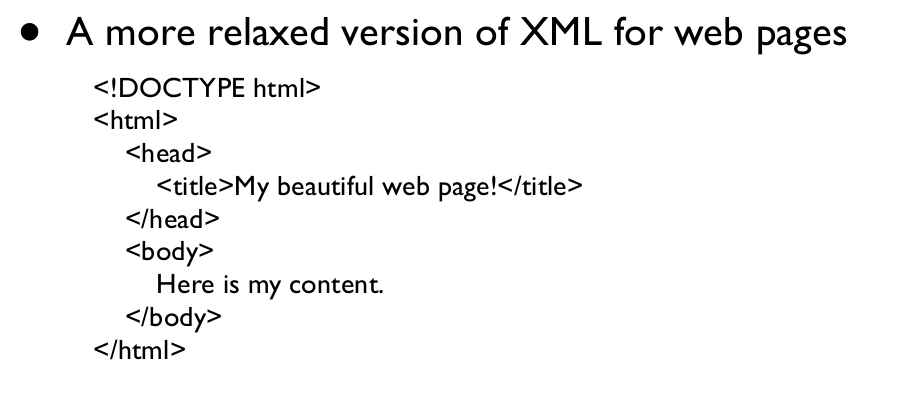
\includegraphics[scale=0.3]{html.png}
    \end{center}
\end{frame}
\begin{frame}{Tags \& Elements}
    \begin{center}
        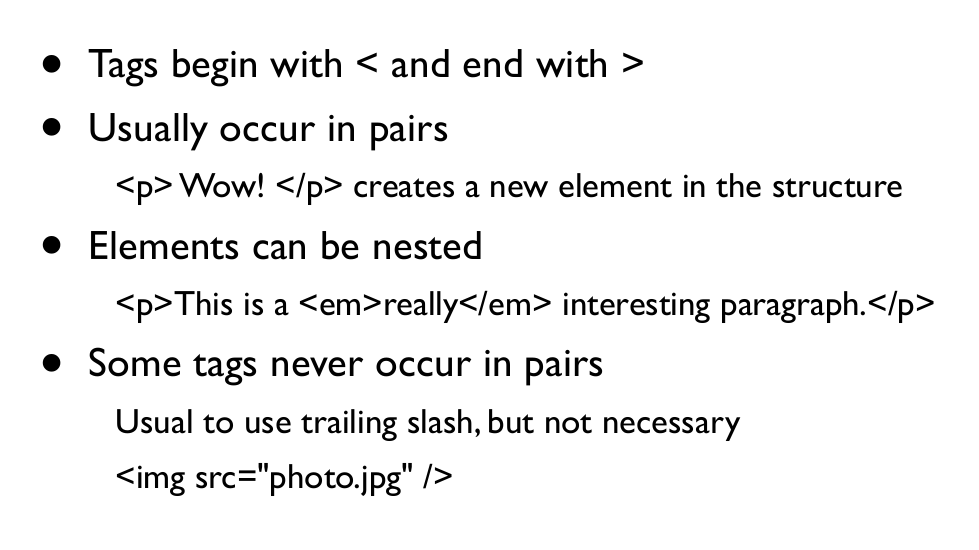
\includegraphics[scale=0.3]{tagsAndElems.png}
    \end{center}
\end{frame}
\begin{frame}{Attributes}
    \begin{center}
        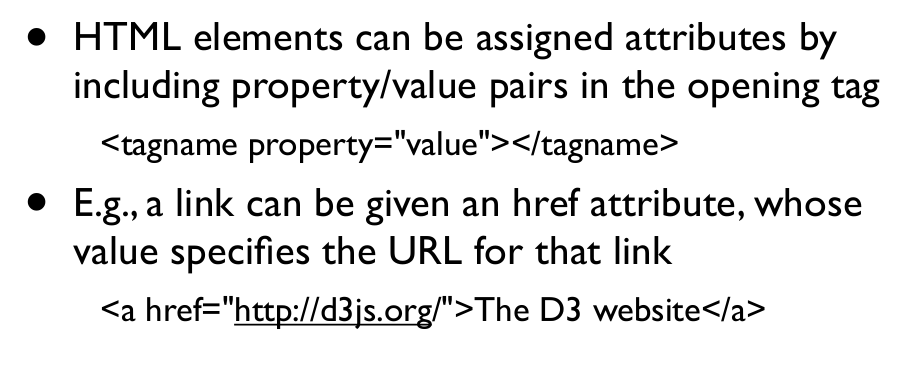
\includegraphics[scale=0.3]{attributes.png}
    \end{center}
\end{frame}
\begin{frame}{Classes and IDs}
    \begin{center}
        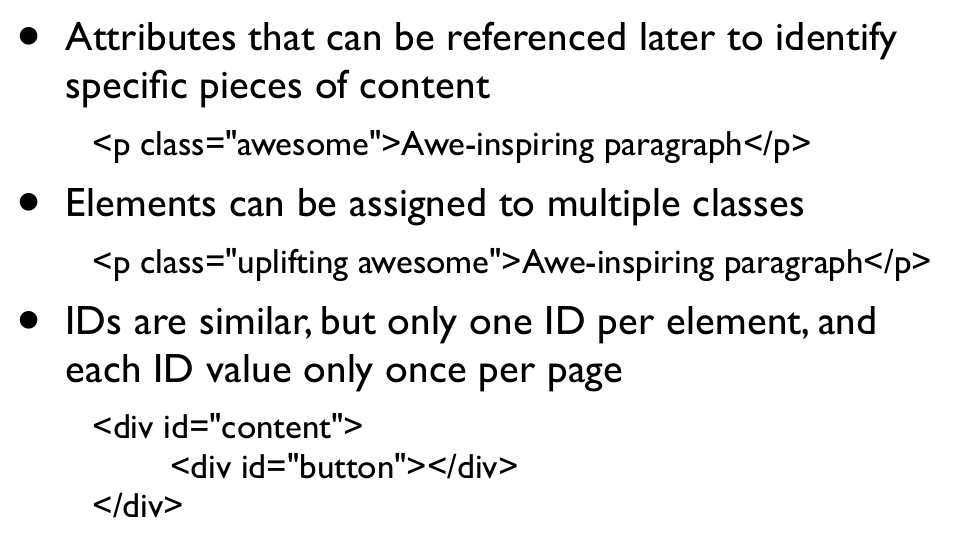
\includegraphics[scale=0.3]{classesAndIDs.png}
    \end{center}
\end{frame}
\begin{frame}{DOM}
    \begin{center}
        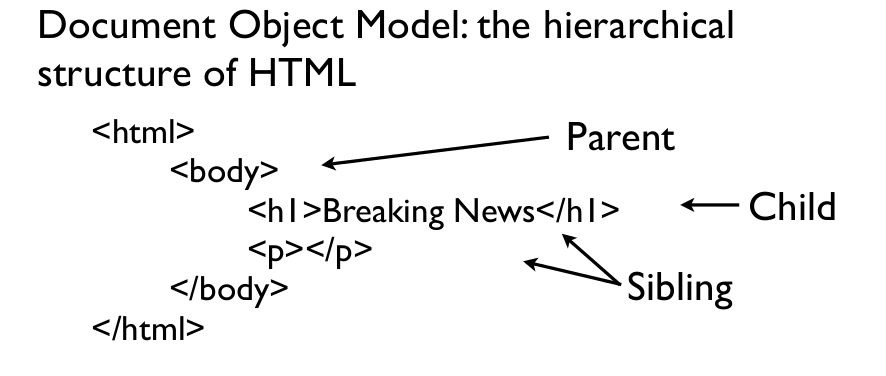
\includegraphics[scale=0.3]{dom.png}
    \end{center}
\end{frame}
\begin{frame}{CSS}
    \begin{center}
        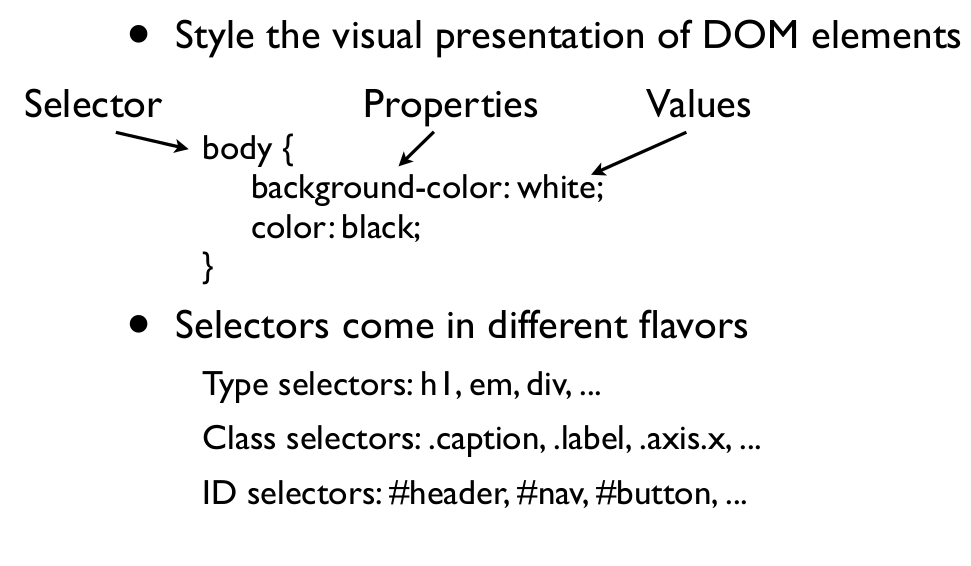
\includegraphics[scale=0.3]{css.png}
    \end{center}
\end{frame}
\begin{frame}{Referencing CSS}
    \begin{center}
        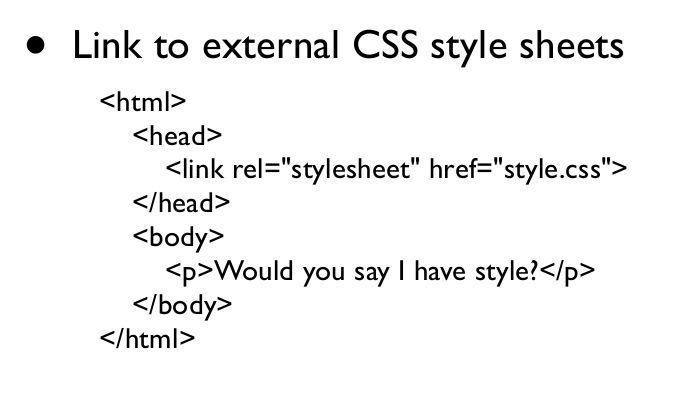
\includegraphics[scale=0.3]{refCSS.png}
    \end{center}
\end{frame}

\section{Web Scraping}
\begin{frame}{} 
    \begin{center}
        \thblue{Web Scraping}
    \end{center}
\end{frame}

\begin{frame}{Web Scraping\footnote{Wikipedia}}
    \begin{center}  
        ``Data scraping is a technique in which a computer program extracts data from human-readable output coming from another program.

        Web pages are built using text-based mark-up languages (HTML and XHTML), and frequently contain a wealth of useful data in text form.  However, most web pages are designed for human end-users and not for ease of automated use.  Because of this, tool kits that scrape web content were created. A web scraper is an API to extract data from a web site.'' 
    \end{center}
\end{frame}


\begin{frame}{Inspecting Web Pages}
    \begin{itemize}
        \item Chrome: DevTools 
        \item Firefox: Developer Tools, Firebug
        \item Safari and Internet Explorer
    \end{itemize}
\end{frame}

\begin{frame}{} 
    \begin{center}
        \thblue{Chrome Developer Tools Demo}
    \end{center}
\end{frame}

\begin{frame}{Web Scraping in Python}
    \begin{itemize}
        \item HTTP Requests: urllib2, requests
        \item HTML Parsing: lxml, beautifulsoup, pattern
        \item Crawling: Scrapy
        \item Controlling Browsers: Selenium/WebDriver
        \item Headless Browsers: PhantomJS
    \end{itemize}
\end{frame}

\begin{frame}{CSS Selectors\furl{http://codylindley.com/jqueryselectors/}}
    \begin{itemize}
        \item '*' : Selects all elements
        \item 'p' : Select all p tags
        \item '\#myid' : Select element with id=myid
        \item '.myclass' : Select elements with class=myclass 
        \item 'p \#myid .myclass' : Union of all the selections
        \item 'div code': Find all code tags inside a div
        \item 'li $>$ ul': Select all ul inside li (first level only)
        \item 'strong + em': Select all em that is immediately preceded by strong
        \item 'prev ~ siblings': Selects all sibling elements that follow after the "prev" element, have the same parent, and match the filtering "siblings" selector. 
    \end{itemize}
\end{frame}
\begin{frame}{CSS Selectors\furl{http://codylindley.com/jqueryselectors/}}
    \begin{itemize}
        \item 'li[class]' : all li with attribute class
        \item ~ [a="b"]: All elements with attribute with name 'a' with value 'b'
        \item 'li:first' : First element of li
        \item 'li:first-child' : First child of li
        \item 'li:even' : Even elements of li
        \item ':text' : All text boxes
    \end{itemize}
\end{frame}

\begin{frame}{Crawling and Spiders}

    wget -mk -w 20 http://www.example.com/
    
    \begin{itemize}
        \item -m : Mirror a website
        \item -k : convert urls to point to local files
        \item -w : Delay between requests. 20 = 20 seconds, 20m $=>$ 20 minutes and so on 
        \item -r : recursive download 
        \item -p : download all files that are necessary to properly display a given HTML page.
        \item -c : continue a incomplete download
        \item --tries : Number of retries
        \item --reject, -A : File types to reject and accept
    \end{itemize}
\end{frame}


\begin{frame}[fragile]
    \frametitle{Scrapy\furl{http://scrapy.org/}}
\begin{verbatim}
from scrapy import Spider, Item, Field

class Post(Item):
    title = Field()

class BlogSpider(Spider):
    name, start_urls = 'blogspider', 
                ['http://blog.scrapinghub.com']

    def parse(self, response):
        return [Post(title=e.extract()) 
                for e in response.css("h2 a::text")]
\end{verbatim}
\end{frame}


\begin{frame}{Web Driver}
    \begin{itemize}
        \item Originally a tool for automating testing of web applications
        \item Now a W3C standard (\url{http://w3c.github.io/webdriver/webdriver-spec.html})
        \item Interface to Selenimum and WebDriver in Python
    \end{itemize}
\end{frame}

\begin{frame}[fragile]
    \frametitle{Selenium WebDriver\furl{https://selenium-python.readthedocs.org/}}
\begin{verbatim}
from selenium import webdriver
from selenium.webdriver.common.keys import Keys

driver = webdriver.Firefox()
driver.get("http://www.python.org")
elem = driver.find_element_by_name("q")
elem.send_keys("pycon")
elem.send_keys(Keys.RETURN)
\end{verbatim}
\end{frame}

\begin{frame}{PhantomJS\furl{https://github.com/ariya/phantomjs}}
    \begin{itemize}
        \item Scriptable Headless WebKit
        \item Automating web related workflow
        \item Use Cases:
        \begin{itemize}
            \item Headless web testing
            \item Page automation.
            \item Screen capture. 
            \item Network monitoring. 
        \end{itemize}
    \end{itemize}
\end{frame}


\begin{frame}{CasperJS\furl{http://casperjs.org/}}
    \begin{itemize}
        \item Navigation scripting and testing utility
        \item Built for PhantomJS
        \item Easy to define full navigation scenarios
        \item Syntactic sugar to make life very easy
    \end{itemize}
\end{frame}


\begin{frame}{} 
    \begin{center}
        \thblue{IMDB Web Scraping Demo}
    \end{center}
\end{frame}
\begin{frame}{} 
    \begin{center}
        \thblue{Facebook Web Scraping Demo}
    \end{center}
\end{frame}


\section{Summary}
\begin{frame}{Summary}

\tblue{Major Concepts:}
\begin{itemize}
    \item Data Collection and Scraping
    \item Tools and Techniques
\end{itemize}
\end{frame}

\begin{frame}{Slide Material References}

\begin{itemize}
    \item Slides from Harvard CS 109 (2013)
    \item Slides by Jeff Leek
    \item Also see slide footnotes
\end{itemize}
\end{frame}


\end{document}

